\ifx\allfiles\undefined
\documentclass[conference]{IEEEtran}
\usepackage{graphicx}
\usepackage[]{subfigure}
\begin{document}
\title{job mapping evaluation (golfgraph)}
\author{huyao}
\date{}
\maketitle
\else
\chapter{job mapping of golfgraph}
\fi
\section{Performance Evaluation of Supercomputer's Networks}
\subsection{Job Mapping}

\subsubsection{Application Performance}

We use a discrete-event simulation framework, SimGrid (v3.12)~\cite{SimGrid}, to evaluate the performance of parallel application benchmarks,  which include Block Tri (BT), Conjugate Gradient (CG), Fast Fourier (FT), Multi-Grid (MG) and Scalar Penta (SP) taken from NAS parallel benchmarks~\cite{benchmark}, Matrix Multiplication (MM) and Graph500.   
We configure SimGrid so that each switch has a 100ns delay, switches and compute nodes are interconnected via the links with 100Gbps bandwidth each, and each compute node has a 5TFlops computation power. 
For realistic simulation time, we use Class B as the problem size of BT, CG, FT, SP and MM, use Class A as the problem size of FT, and use Class Tiny as the problem size of Graph500.

In the simulation, we assume the minimal routing using the Dijkstra algorithm on target 256-node interconnection networks, which are divided into two groups: degree-4 and degree-8.
For each group we evaluate the performance on Torus ($16 \times 16$ for degree-4 and $4 \times 4 \times 4 \times 4$ for degree-8), Random and GolfGraph.

\begin{figure}[tb]
	\centering
	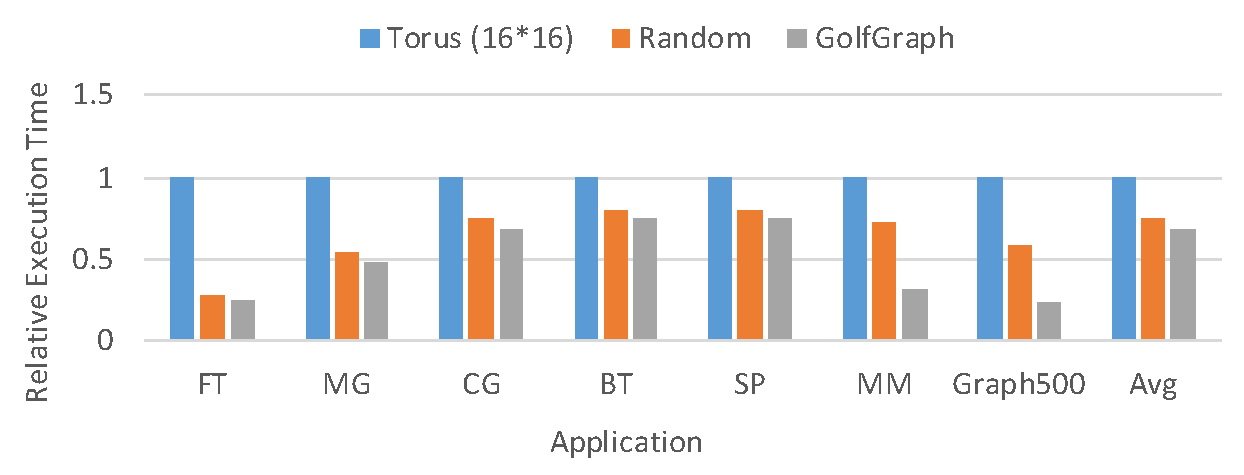
\includegraphics[width=8cm]{ps/exec-d4.pdf}
	\caption{Execution time of benchmark applications (nodes = 256, degree = 4).}
	\label{fig:exec-d4}
\end{figure}

\begin{figure}[tb]
	\centering
	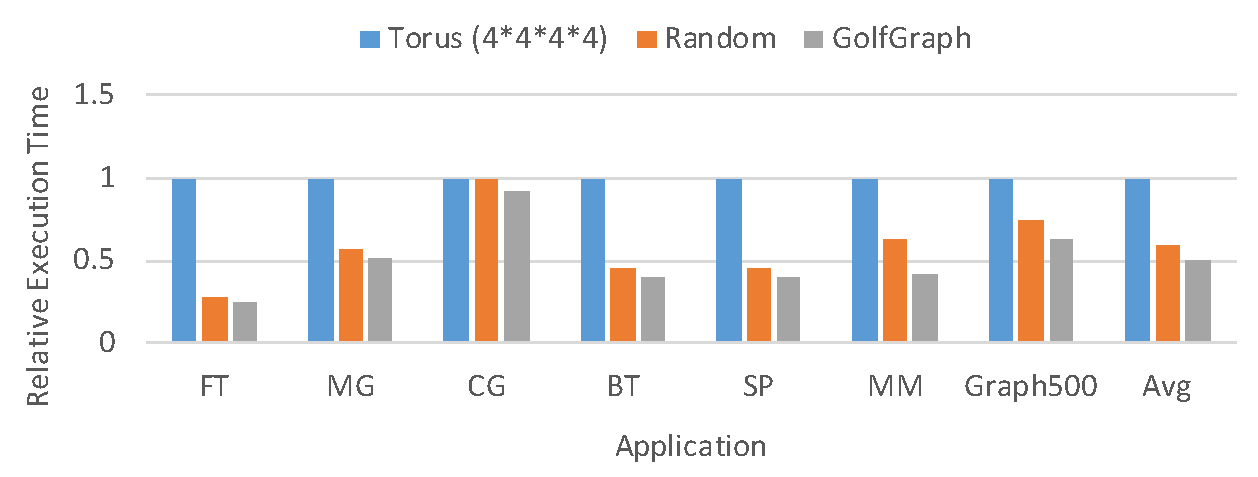
\includegraphics[width=8cm]{ps/exec-d8.pdf}
	\caption{Execution time of benchmark applications (nodes = 256, degree = 8).}
	\label{fig:exec-d8}
\end{figure}

\subsubsection{Scheduling Performance}

We developed an event-driven HPC simulator written in Python 2.7 in a machine with Intel i7-1165G7 (2.80GHz) CPU and 16GiB Memory to model application mapping over target 1024-node interconnection networks. 
We evaluate the performance of application mapping and job scheduling with a compound workload of various NPB applications~\cite{NPB} and several real-world HPC workload traces~\cite{wm}.

The network competitors are the same as those in the previous subsection: Torus ($4 \times 4 \times 8 \times 8$), Random and GolfGraph, which have the same degree 8.
We use a contiguous mapping policy on target interconnection networks, which allocates a job to the available compute nodes whose attached switches are directly connected. 
In this case, the end-to-end hop count can be relatively reduced, which leads to a compact low-diameter embedded topology for job execution.

We assume that each application occupies a fixed number of compute nodes during runtime by applying a common approach to model parallel ``rigid" jobs.
We use FCFS (First Come First Served) together with EASY backfilling~\cite{easy} as the job queuing policy.
We employ the following two workload types:
\begin{itemize}
\item 
\emph{Compound Workload of NPB Application}: 
The workload is composed of the above NPB applications, and each job randomly specifies the number (4, 16, 64 or 256) of required compute nodes.
We generate $n = 2000$ jobs as a workload with random arrival timings for a \emph{Poisson} process with $\lambda = \frac{n}{100}$. 
\item 
\emph{PWA Workload Traces}: 
We use real-world supercomputer workload traces of user jobs by employing the parallel workloads archive (PWA) datasets~\cite{PWA}. 
Each archive in the PWA datasets uses a standard workload format, which concerns the arrivals of jobs and their basic resource requirements, namely the number of compute nodes and the processing time. 
In the evaluation, we exemplarily use four PWA datasets: SDSC-Par, NASA-iPSC, SDSC-SP2 and HPC2N.
More detailed information about the PWA datasets can be found in \cite{pwa2014}.

\begin{figure}[tb]
	\centering
	\subfigure[Average response time (s)]{
	  \label{fig:subfig:npb-time} 
	  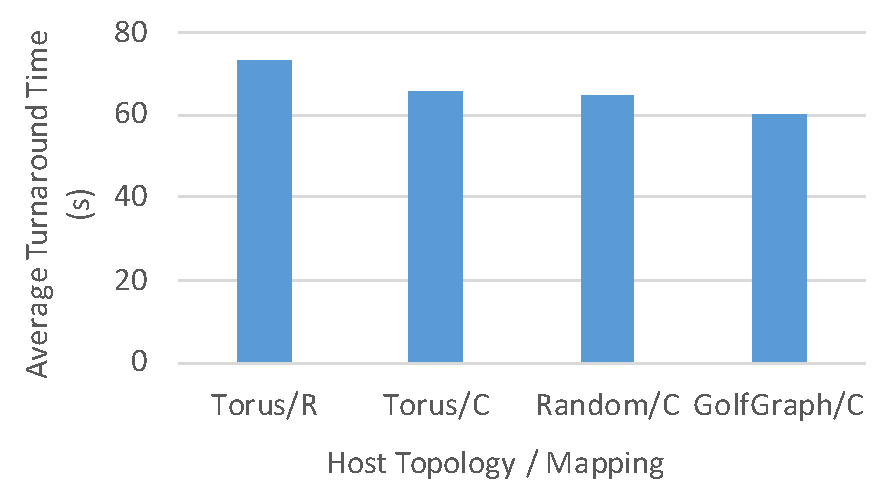
\includegraphics[width=4cm]{ps/npb-time.pdf}}
	% \hspace{0.1in} 	
	\subfigure[Resource utilization]{
	  \label{fig:subfig:npb-uti} 
	  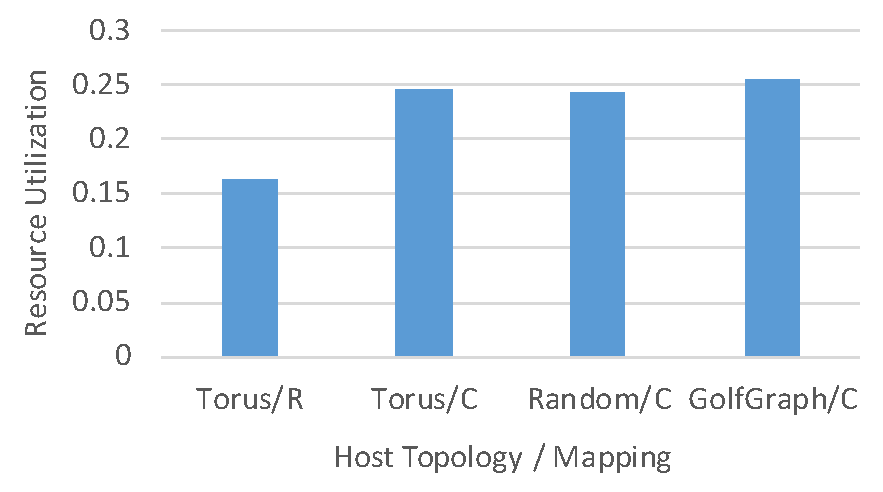
\includegraphics[width=4cm]{ps/npb-uti.pdf}}        
	\caption{Job scheduling performance using NPB applications on 1024-node interconnection networks.}
	\label{fig:npb} 
\end{figure}

\begin{figure}[tb]
	\centering
	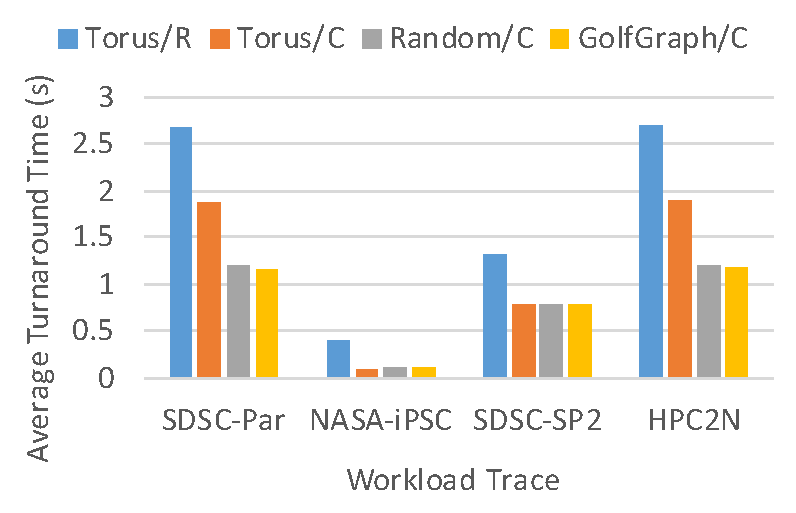
\includegraphics[width=8cm]{ps/pwa-time.pdf}
	\caption{Average turnaround time using PWA workload traces on 1024-node interconnection networks.}
	\label{fig:pwa-time}
\end{figure}

\begin{figure}[tb]
	\centering
	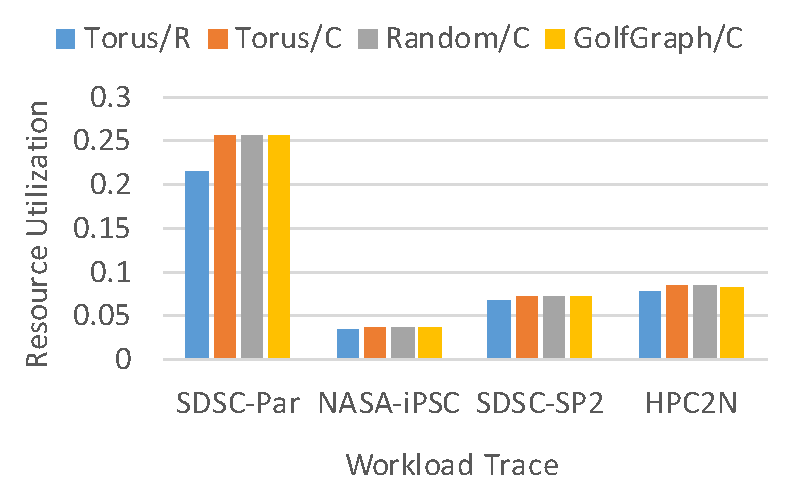
\includegraphics[width=8cm]{ps/pwa-uti.pdf}
	\caption{Resource utilization using PWA workload traces on 1024-node interconnection networks.}
	\label{fig:pwa-uti}
\end{figure}

\end{itemize}

\ifx\allfiles\undefined
\end{document}
\fi


